\chapter{Evaluation}\label{evaluation}

\blindtext[1]

\newpage

\textbf{Plan:}

Große Fragen:

\begin{itemize}
\tightlist
\item
  Spielbar? User Tests?
\item
  Nur im LAN, oder auch übers Internet?
\item
  Welche Latenz war angestrebt? Erreicht?
\end{itemize}

Faktenbasiert, Metriken:

\begin{itemize}
\tightlist
\item
  Emulatior-FPS

  \begin{itemize}
  \tightlist
  \item
    Emulator kann FPS anzeigen
  \item
    Code so anpassen, dass die FPS durch JavaScript über eine API
    zugänglich sind und diesen Wert auslesen
  \item
    Für den Test bietet sich Selenium an

    \begin{itemize}
    \tightlist
    \item
      Automatisiert
    \item
      Mehrere Browser, Dienstleister: Saucelabs, BrowserStack
    \item
      Schritte:

      \begin{itemize}
      \tightlist
      \item
        Match hosten
      \item
        Spiel hochladen
      \item
        Über N Zeiteinheiten FPS auslesen (bzgl. Statistik Tipps
        einholen)
      \end{itemize}
    \end{itemize}
  \end{itemize}
\item
  Netzwerk-Metriken von WebRTC

  \begin{itemize}
  \tightlist
  \item
    Automatisierung nicht ganz einfach, weil zwei Browser kommunizieren
    müssten. Unbekannt, ob Selenium das kann (also ein ``Pair spawnen'',
    oder sowas)
  \item
    Auslesen ist über das Control-Protokoll sehr gut machbar. Alle
    WebRTC-fähigen Browser haben dafür meist eine eigene Ansicht, auf
    der Debug-Informationen bzgl. WebRTC angezeigt werden
  \end{itemize}
\end{itemize}

\textbf{Weitere Ideen:}

\begin{itemize}
\tightlist
\item
  WebRTC vs.~WebSockets

  \begin{itemize}
  \tightlist
  \item
    Wenn LAN-Spiel: Welchen Vorteil bringt WebRTC? (Wie viel weniger
    Latenz?)
  \end{itemize}
\item
  Emulator: emscripten-Backends vergleichen. asm.js vs.~WebAssembly.
  Emulator funktioniert mit beidem in den zu unterstützenden Browsern
  (Chrome, Firefox). Bringt es Vorteile? Bessere Framerate? Wie viel
  besser? Andere Metriken?
\end{itemize}

\section{Aufbau der Messumgebung}\label{aufbau-der-messumgebung}

\section{Ergebnisse und
Beobachtungen}\label{ergebnisse-und-beobachtungen}

https://www.sharelatex.com/learn/Pgfplots\_package

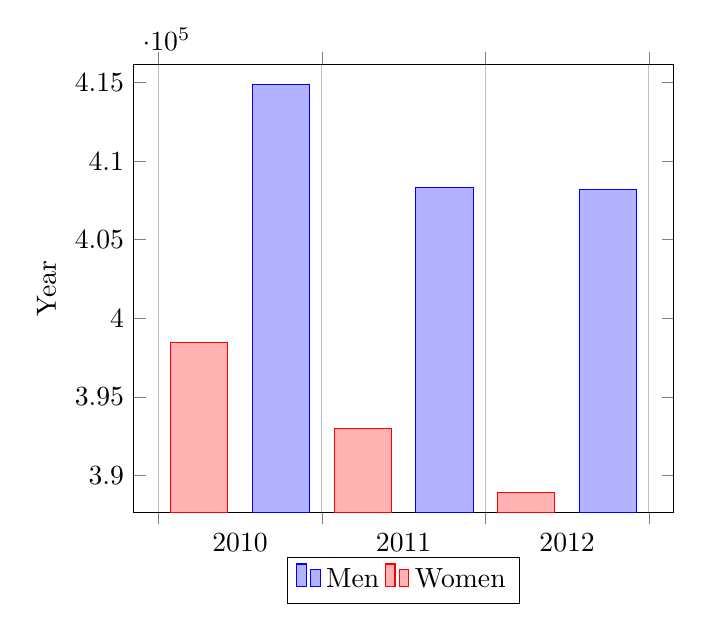
\begin{tikzpicture}
\begin{axis}[
    x tick label style={
        /pgf/number format/1000 sep=},
    ylabel=Year,
    enlargelimits=0.05,
    legend style={at={(0.5,-0.1)},
    anchor=north,legend columns=-1},
    ybar interval=0.7,
]
\addplot 
    coordinates {(2012,408184) (2011,408348)
         (2010,414870) (2009,412156)};
\addplot 
    coordinates {(2012,388950) (2011,393007) 
        (2010,398449) (2009,395972)};
\legend{Men,Women}
\end{axis}
\end{tikzpicture}

\section{Diskussion und Bewertung}\label{diskussion-und-bewertung}
